% !TeX spellcheck = en_US
%\documentclass[11pt,a4paper]{article}
\documentclass[11pt
  , a4paper
  , article
  , oneside
%  , twoside
%  , draft
]{memoir}

\usepackage{control}
\usepackage{kotex}
\usepackage[numbers]{natbib}
%\usepackage[pdftex]{graphicx}
%\DeclareGraphicsExtensions{.pdf,.png,.jpg}
\begin{document}

\newcommand{\technumber}{
  Digital Signal Processing using MATLAB\\
  Document 1: 2016-03-26}
\title{\textbf{Digital Signal Processing: 실습 9 \\
		제4장 z-변환 \\}}

\author{이상일\thanks{silee7103@ibs.re.kr} \\

  학번: 201460437\\
  Computer Engineering, Chungnam National University 
}
\date{\today}

\renewcommand{\maketitlehooka}{\begin{flushright}\textsf{\technumber}\end{flushright}}
%\renewcommand{\maketitlehookb}{\centering\textsf{\subtitle}}
%\renewcommand{\maketitlehookc}{C}
%\renewcommand{\maketitlehookd}{D}

\maketitle

\begin{abstract}
MATLAB을 사용한 Digital Signal Processing에 대한 실습과제에 대한 Documents를 구성한다.
\end{abstract}

\chapter{Example 4-14:}

\begin{lstlisting}[style=termstyle]
%Example 4.14

b = [1,0,0]; a = [1, -3/2,1/2];
n = [0:7]; x = (1/4).^n; 
xic = [1,-2];

format long;

y1 = filter(b,a,x,xic)

y2 =  (1/3)*(1/4).^n+(1/2).^n+(2/3)*ones(1,8)

Y = [4,10]; xic = filtic(b,a,Y)
\end{lstlisting}

\begin{figure}[h!]
	\centering
	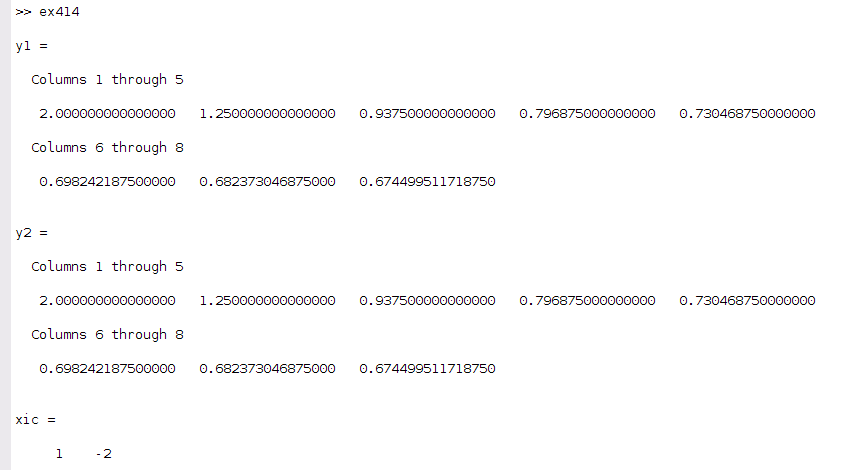
\includegraphics[width=0.6\textwidth,height=0.4\textwidth]{./images/ex414.png}
	\caption{Example 4.14 Result}
	\label{fig:Example 4.14 Result}
\end{figure}

\chapter{Example 4-15:}
\subsection{Example 4-15a}
\begin{lstlisting}[style=termstyle]
Example 4.15a

b=[1,1,1]/3; a=[1, -0.95, 0.9025];

Y = [-2,-3]; X = [1,1]; xic = filtic(b,a,Y,X)

bxplus = [1, -0.5]; axplus = [1,-1,1];
ayplus = conv(a,axplus)
byplus = conv(b,bxplus) + conv(xic, axplus)

[R,p,C]= residuez(byplus, ayplus)

Mp = abs(p), Ap=angle(p)/pi\end{lstlisting}

\begin{figure}[h!]
	\centering
	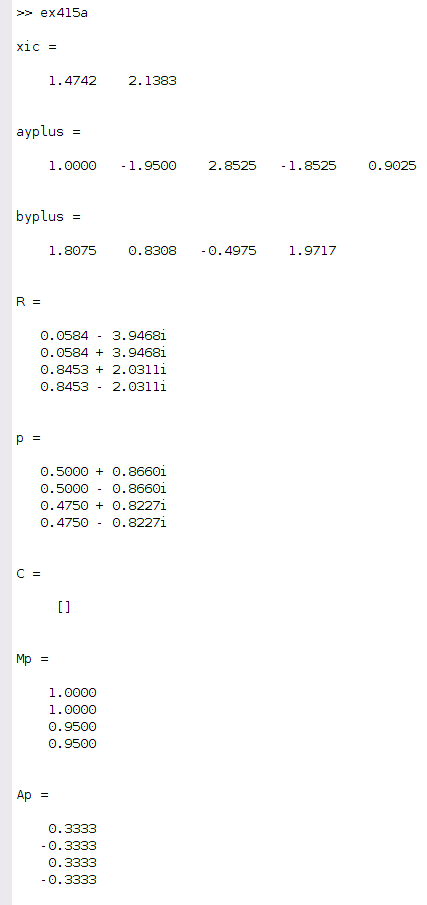
\includegraphics[width=0.6\textwidth,height=0.4\textwidth]{./images/ex415a.png}
	\caption{Example 4.15a Result}
	\label{fig:Example 4.15a Result}
\end{figure}

\subsection{4-15b}
\begin{lstlisting}[style=termstyle]
Example 4.15b

n = [0:7]; x = cos(pi*n/3); y = filter(b,a,x,xic)
A = real(2*R(1)); B = imag(2*R(2)); C = real(2*R(3)); D = imag(2*R(4));

y = A*cos(pi*n/3) + B*sin(pi*n/3) + ((0.95).^n).*(C*cos(pi*n/3)+D*sin(pi*n/3))
\end{lstlisting}

\begin{figure}[h!]
	\centering
	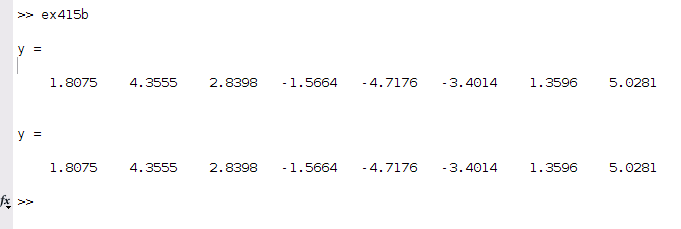
\includegraphics[width=0.5\textwidth,height=0.3\textwidth]{./images/ex415b.png}
	\caption{Example 4.15b Result}
	\label{fig:Example 4.15b Result}
\end{figure}


\chapter{연습문제 4.24: }
\section{4.24-1: }

\begin {equation}
H(z) = K\frac{(z-1)(z+1)(z-i)(z+j)}{(z-0.9)(z+0.9)(z-j0.9)(z+j0.9)} = K\frac{1-z^{-4}}{1-0.6561z^{-4}}, |z|>0.9 \nonumber
\end {equation}

따라서,
\begin {equation}
1 = H(z) = K\frac{1-e^{j\pi}}{1-0.6561e^{j\pi}} = K * 1.2077 => K = 0.8281 \nonumber
\end {equation}

\begin {equation}
H(z) = \frac{0.8281(1-z^{-4})}{1-0.6561z^{-4}}, |z| > 0.9 \nonumber
\end {equation}


\section{4.24-2: }
\begin {equation}
H(z) = \frac{0.8281(1-z^{-4})}{1-0.6561z^{-4}} = \frac{Y(z)}{X(z)} \nonumber
\end {equation}

따라서,
\begin {equation}
y(n) = 0.8281x(n) - 0.8281x(n-4) + 0.6561y(n-4) \nonumber
\end {equation}

\section{4.24-3: }
\begin {equation}
H(z) = \frac{1-[cos(\pi/4)]z^{-1}}{1-[2cos(\pi/4)]z^{-1} + z^{-2}} = \frac{1-\frac{1}{\sqrt{2}}z^{-1}}{1-\sqrt{2}z^{-1}+z^{-2}}   \nonumber
\end {equation}

따라서,

\begin {equation}
\begin {split}
Y(z)=H(z)X(z) = (\frac{0.8281(1-z^{-4})}{1-0.6561z^{-4}})(\frac{1-\frac{1}{\sqrt{2}}z^{-1}}{1-\sqrt{2}z^{-1}+z^{-2}}) &\\
= \frac{1-\frac{1}{\sqrt{2}}z^{-1}}{1-\sqrt{2}z^{-1}+z^{-2}}-\frac{0.0351}{1-0.9z^{-1}}-\frac{0.0509}{1+0.9z^{-1}} + \frac{-0.0860 - 0.1358z^{-1}}{1-0.81z^{-2}}, |z| >1    \nonumber
\end{split}
\end {equation}

따라서,
\begin {equation}
y_{ss}(n)= cos(\pi n/4) \nonumber
\end {equation}

\section{4.24-4: }
\begin {equation}
\begin {split}
Y_{u}(z)=-\frac{0.0351}{1-0.9z^{-1}}-\frac{0.0509}{1+0.9z^{-1}} - 0.0860\frac{1}{1-0.81z^{-2}} - 0.1509\frac{0.9z^{-1}}{1-0.81z^{-2}}, |z| >1    \nonumber
\end{split}
\end {equation}

따라서,
\begin {equation}
\begin {split}
Y_{u}(n)= -0.0351(0.9)^nu(n) - 0.0509(-0.9)^nu(n) - 0.086(0.9)^n cos(\pi n/2)u(n) & \\
-0.1509(0.9)^n sin(\pi n/2)u(n)    \nonumber
\end{split}
\end {equation}


\chapter{연습문제 4.25: }
주어진 식에서,
\begin {equation}
\begin {split}
Y^+(z) = 0.81[y(-2)+y(-1)z^{-1}+z^{-2}Y^+(z)] + X^+(z) -[x(-1)+z^{-1}X^+(z)]  &\\ 
= 0.81z^{-2}Y^+(z)+[1-z^{-1}]X^+(z) + [0.81y(-2)+[0.81y(-2) - x(-1)] + 0.81y^{-1}z^{-1}]
\nonumber
\end{split}
\end {equation}

이를 정리하면,
\begin {equation}
\begin {split}
Y^+(z) = (\frac{1-z^{-1}}{1-0.81z^{-1}})(\frac{1}{1-0.7z^{-1}}) + \frac{0.1914+1.62z^{-1}}{1-0.81z^{-1}}
\nonumber
\end{split}
\end {equation}

전개하여 정리하면,
\begin {equation}
\begin {split}
Y^+(z) = 2 + \frac{0.4642}{1-0.81z^{-1}} + \frac{2.7273}{1-0.7z^{-1}}
\nonumber
\end{split}
\end {equation}

역 z-변화를 하면,
\begin {equation}
\begin {split}
y(n) = 2\delta(n) + 0.4642(0.81)^nu(n)+2.7273(0.7)^nu(n)
\nonumber
\end{split}
\end {equation}

\begin{lstlisting}[style=termstyle]
b1 = [1 -1]; nb1 = [0 1]; 
a11 = [1 0 -0.81]; 
na11 = [0 1 2]; a12 = [1 -0.7];
na12 = [0 1]; 
[a1,na1] = conv_m(a11,na11,a12,na12);

b2 = [0.1914 1.62]; nb2 = [0 1]; a2 = [1 0 -0.81]; na2 = [0 1 2];
[bnr1,nbnr1] = conv_m(b1,nb1,a2,na2); 
[bnr2,nbnr2] = conv_m(b2,nb2,a1,na1);

[b,nb] = sigadd(bnr1,nbnr1,bnr2,nbnr2); [a,na] = conv_m(a1,na1,a2,na2);
[R,p,k] = residuez(b,a)

n = [0:20]; x = 0.7.^n; xic = [0.1914 1.62];

yb1 = filter(b1,a11,x,xic);
yb2 = R(1)*((p(1)).^n)+R(3)*((p(3)).^n)+R(5)*((p(5)).^n);

error = max(abs(yb1-yb2))
\end{lstlisting}


\begin{figure}[h!]
	\centering
	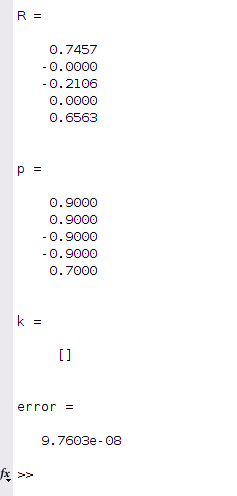
\includegraphics[width=0.5\textwidth,height=0.3\textwidth]{./images/p425.png}
	\caption{Example 4.25 Result}
	\label{fig:Example 4.25 Result}
\end{figure}


\chapter{연습문제 4.26: }
주어진 식에서,

\begin {equation}
\begin {split}
Y^+(z) - 0.4y(-1) -0.4z^{-1}Y^+(z) - 0.45y(-2) - 0.45y(-1)z^{-1} - 0.45z^{-2}Y^+(z) &\\
 = 0.45X^+(z) + 0.4x(-1)+0.4z^{-1}X^+(z)-x(-2)-x(-1)z^{-1}-z^{-2}X^+(x)   \nonumber
\end{split}
\end {equation}


입력신호에 대한 역 z-변환를 대입하면,
\begin {equation}
\begin {split}
Y^+(z)= ()\frac{0.45+0.4z^{-1}-z^{-2}}{1-0.4z^{-1}-0.45z^{-2}})(\frac{2}{1-z^{-1}}+\frac{1}{1-0.5z^{-1}}) &\\
+ \frac{0.15-2z^{-1}}{1-0.4z^{-1}-0.45z^{-2}}
\nonumber
\end{split}
\end {equation}

이를 정리하면,
\begin {equation}
\begin {split}
Y^+(z)= \frac{-2}{1-z^{-1}}+\frac{2.116}{1-0.9z^{-1}}+\frac{1.7188}{1-0.5z^{-1}}-\frac{0.3304}{1+0.5z^{-1}}
\nonumber
\end{split}
\end {equation}

역 z-변환를 취하면,
\begin {equation}
\begin {split}
y(n)= [-2 + 2.1116(0.9)^n + 1.7188(0.5)^n - 0.3303(-0.5)^n]u(n)
\nonumber
\end{split}
\end {equation}

\section{4.26-1:}
\begin {equation}
\begin {split}
y_{tr}(n)= [2.1116(0.9)^n + 1.7188(0.5)^n - 0.3303(-0.5)^n]u(n)
\nonumber
\end{split}
\end {equation}

\section{4.26-2:}
\begin {equation}
\begin {split}
y_{ss}(n)= -2
\nonumber
\end{split}
\end {equation}

\section{4.26-3:}
\begin {equation}
\begin {split}
Y^+_{zi}(z)=\frac{0.15 -2z^{-1}}{1-0.4z^{-1}-0.45z^{-2}} = \frac{-1.3321}{1-0.9z^{-1}} + \frac{1.4821}{1+0.5z^{-1}} 
\nonumber
\end{split}
\end {equation}

\begin {equation}
\begin {split}
y^+_{zi}(n)= [-1.3321(0.9)^n + 1.4821(-0.5)^n]u(n)
\nonumber
\end{split}
\end {equation}

\section{4.26-4:}
\begin {equation}
\begin {split}
Y^+_{zs}(z)=\frac{1.35+0.3z^{-1}-3.8z^{-2}+2z^{-3}}{(1-0.9z^{-1})(1+0.5z^{-1})(1-z^{-1})(1-0.5z^{-1})} &\\ = \frac{-2}{1-z^{-1}} + \frac{3.4438}{1-0.9z^{-1}} +\frac{1.7187}{1-0.5z^{-1}} - \frac{1.8125}{1+0.5z^{-1}} 
\nonumber
\end{split}
\end {equation}

\begin {equation}
\begin {split}
y^+_{zs}(n)= [-2 + 3.4438(0.9)^n + 1.7187(0.5)^n - 1.8125(-0.5)^n]u(n)
\nonumber
\end{split}
\end {equation}

\end{document}

